\documentclass{article}
\usepackage[utf8]{inputenc}
\usepackage{graphicx} % Required for inserting images
\usepackage{amsmath}
\usepackage[brazil]{babel}

\title{RELATÓRIO II: COMPARAÇÃO DE PERFORMANCE ÓTIMO VS APROXIMADO PARA PD}
\author{
    Ryan Augusto Brandão Salles - 221008436\\
    Víctor Moreira Almeida - 221008481\\
}

\date{Fevereiro de 2024}

\begin{document}

\maketitle

\section{Introdução}
    Essa seção visa trazer alguns assuntos introdutórios, mais precisamente, situar o leitor sobre o que se trata esse documento, qual o trabalho que busca ser realizado e qual exatamente seria sua motivação, além de demais especificidades de caráter estritamente introdutório ao teor do que será tratado nesse relatório.

\subsection{O que é esse documento}
    Esse documento é um relatório que sumariza os resultados obtidos durante a implementação e testagem de algoritmos de aproximação para o problema da Mochila (Knapsack) na disciplina de Projeto de Algoritmos durante o semestre 2024.2. Além disso, são detalhadas as abordagens utilizadas na implementação desses algoritmos.\\
    
    Mais especificamente, o relatório apresenta uma comparação entre algoritmos exatos e heurísticos, com ênfase na otimização do problema da mochila utilizando Programação Dinâmica e sua comparação com uma abordagem gulosa (Greedy). Detalhes sobre esses algoritmos podem ser encontrados na seção \ref{algoritmos}.\\

    Ademais, o algoritmo foi escolhido por apresentar um equilíbrio entre facilidade de implementação e possíveis \textit{insights}, ou seja, o algoritmo ótimo e sua aproximação apresentam bom valor de aprendizado de um ponto de vista acadêmico sem a necessidade de um tempo de investimento longo\\

\subsection{O que não é esse documento}
    Esse documento não tem como objetivo ser uma pesquisa formal sobre a otimização do problema da Mochila (Knapsack) nem apresentar uma implementação completa e definitiva. Trata-se apenas de um experimento exploratório realizado pela dupla, cujo intuito é compartilhar observações e resultados que possam ser de interesse para seus colegas e avaliadores.
    
    Além disso, este relatório não pretende ser uma prova definitiva de superioridade da Programação Dinâmica para problemas que involvem decisões a cada etapa e tampouco pretende provar que uma aproximação é sempre melhor para aplicações com restrições estritas de tempo de entrega do resultado. A eficiência de cada método depende do contexto e das restrições do problema, sendo necessário um estudo mais aprofundado para determinar a melhor abordagem em cada caso específico.

\subsection{Justificativa I: possibilidade de melhor desempenho de tempo e suas consequências}
    O desempenho de algoritmos de otimização pode ser crucial para problemas de grande escala. Melhor eficiência pode significar a diferença entre obter uma solução em poucas horas ou precisar de anos de processamento. No caso do problema da Mochila (Knapsack), técnicas como Programação Dinâmica podem oferecer ganhos significativos em relação a abordagens heurísticas, tornando possível resolver instâncias maiores de forma mais viável.\\

    Na mesma moeda, o consumo de memória atrelado às decisões necessárias para obter a resposta otima e montar a matriz de decisão podem tornar inviável o uso de um algoritmo da família da Programação Dinâmica para certas aplicações, tais como jogos eletrônicos.\\

    Buscamos, portanto, entender onde os algoritmos performam ou falham de acordo com suas características. 
    
\subsection{Justificativa II: interesse acadêmico e lúdico}
    Algoritmos acadêmicos são tradicionalmente implementados de maneira sequencial, explorando apenas abordagens clássicas como Programação Dinâmica ou Heurísticas Gulosas. Nosso objetivo foi investigar as diferenças de desempenho entre essas abordagens e compreender melhor seus impactos práticos.\\
    
    Mais especificamente, o algoritmo guloso, apesar de eficiente, nem sempre encontra a solução ótima, enquanto a Programação Dinâmica pode garantir essa optimalidade, ainda que com maior custo computacional. Isso levanta a questão de quão grande é essa diferença na prática e até que ponto vale a pena sacrificar precisão por tempo de execução.

    Além disso, simplesmente parece uma análise interessante e divertida de se realizar, o que por si só já seria uma justificativa válida—caso as \textbf{outras justificativas} não fossem suficientes.


\subsection{Escolha de linguagem}
    A linguagem escolhida para essa implementação foi (novamente) a Python, por duas razões simples:
    \begin{itemize}
        \item simplicidade de uso
        \item disponibilidade de utensílios
        \item facilidade de desenvolvimento rápido
    \end{itemize}
    Onde por "simplicidade de uso" queremos dizer "Nós não precisamos pensar muito em como algo precisa ser feito ou pesquisar sintaxe" e, por "disponibilidade de utensílios" queremos dizer "não é necessário escrever algo tão básico quanto uma lista encadeada ou um método pop, a linguagem já possui isso implementada na biblioteca padrão". O desenvolvimento rápido é meramente uma consequência das outras justificativas\\

\section{Metodologia}
    Para esse experimento, a metodologia utilizada é o seguinte procedimento:
    \begin{enumerate}
        \item implementação dos algoritmos do Knapsack
        \item avaliação da performance
        \item implementação dos algoritmos ótimo e aproximado por greed
        \item avaliação da performance dos algoritmos
        \item comparação de performances e determinação da acurácia do Greedy
    \end{enumerate}
    Esses itens servirão de subtópicos para a metodologia e serão expandidos a seguir.\\
    Demais tópicos além dos enumerados serão adicionados conforme necessidade.\\
    \subsection{Hardware utilizado}
        Antes de iniciar a implementação, é importante definir o hardware que será utilizado para os cálculos, afim de evitar duvidas caso haja discrepância entre os resultados.\\
        Serão utilizados dois computadores:
        \begin{itemize}
            \item Dell G15 5520.
                \begin{itemize}
                    \item OS: Windows 10 Pro 22H2
                    \item CPU: Intel(R) Core(TM) i5-12500H
                \end{itemize}
                
            \item SteamDeck LCD.
                \begin{itemize}
                    \item SteamOS Holo 3.6.20.
                \end{itemize}
        \end{itemize}
    
    \subsection{Implementação dos algoritmos do Knapsack}
        A implementação do algoritmo base consiste em implementar o algoritmo em python inicialmente de forma ótima para idealmente obter um ótimo para comparação posterior com o algoritmo de aproximação. 
    
    \subsection{Avaliação da performance base}
        A avaliação da performance base se dará por rodar o algoritmo obtido na implementação base e observar como a curva de crescimento do tempo de execução se comporta para inputs cada vez maiores. Isso serve 2 propósitos simples:
        \begin{itemize}
            \item Averiguar se a implementação feita foi o mais próxima possível de uma complexidade ótima (cuja negação implica na necessidade de corrigir o algoritmo para o caso ótimo);
        \end{itemize}
        e, certamente,
        \begin{itemize}
            \item Obter a performance que desejamos melhorar com o uso de estratégias de aproximação, mais especificamente, buscamos diminuir o custo computacional à um custo de valor na bolsa do knapsack que deve ser levado em consideração.
        \end{itemize}
        
            Mais especificamente, buscamos descobrir quão próximos do ótimo os algoritmos de aproximação chegam e quanto tempo a menos eles podem custar, assunto do nosso próximo tópico
    
    \subsection{Método de comparação ótimo vs. aprox.}
        Para cada rodagem em um determinado conjunto de dados gerado aleatoriamente. Os algoritmos
        serão comparados a partir da performance 
    \subsection{Conjunto de dados para testagem}
    Utilizaremos a biblioteca time para obter o tempo de execução do algoritmo e um vetor de pares peso-valor, denominado item, gerado durante a execução que utilizará a biblioteca random. Os testes serão os seguintes:
        \begin{enumerate}
            \item 10 itens com 10 de peso máximo na mochila gerados com seed 10
            \item 110 itens com 20 de peso máximo na mochila gerados com seed 110
            \item 210 itens com 30 de peso máximo na mochila gerados com seed 210
        \end{enumerate}
    E assim por diante, aumentando progressivamente o conjunto de dados e a seed por um fator de 100 com a finalização da execução ocorrendo com 9910 itens.
    
    \section{Algoritmos}\label{algoritmos}
    Nesse tópico, serão brevemente explicados os algoritmos implementados, seu funcionamento, objetivo e estratégia de resolução do problema.
    
    \subsection{Knapsack - Versão dinâmica iterativa}
    O algoritmo dinâmico iterativo para o knapsack busca prencher uma matriz $I\ X\ P$, onde I são os itens a serem considerados e P é o peso. Para cada célula da matriz, o algoritmo leva em consideração as seguintes questões sobre o item e o peso:
    \begin{itemize}
        \item Considerando o peso remanescente, é possível colocar esse item na mochila?
        \item Considerando o que foi previamente calculado, vale a pena levar esse item em detrimento de outros itens?
    \end{itemize}
    Respondidas essas perguntas, o algoritmo decide entre levar ou não o item sempre tentando maximizar o valor levado. Como a nossa implementação é a iterativa, sempre são respondidas essas perguntas para versões mais simples do problema em questão e o algoritmo deve aos poucos construir a versão mais completa do problema.\\
    Isso implica em preencher cada célula da matriz, sempre do canto superior esquerdo para o canto inferior direito, onde reside a resposta ótima.\\
    Para determinar quais itens foram pegos, um algoritmo secundário, o finder, é rodado após a geração da matriz. Ao contrário do algoritmo principal, ele roda a partir da célula de resposta e sempre busca responder:
    \begin{itemize}
        \item A célula atual é maior que a célula diretamente superior?
    \end{itemize}
    Se sim, o item da linha específica foi colocado na mochila. Se não, ou seja, a célula diretamente acíma possui o mesmo valor da célula atual, o item não foi pego.
    
    \subsection{Knapsack - Aproximação por estratégia gananciosa/greedy}
    Um algoritmo completamente diferente e certamente mais simples, ele utiliza a estratégia de sortir os itens por uma taxa valor sobre peso, que chamaremos de vsp. Sortidos os itens por vsp, basta coletar os itens com a maior taxa vsp até que:
    \begin{itemize}
        \item não hajam mais itens ou
        \item a mochila esteja cheia
    \end{itemize}
    Sua performance é altamente dependente da velocidade do algoritmo de ordenação utilizado para obter a ordem em qual os itens devem ser processados. O restante é simplesmente preencher a mochila para gerar a resposta, uma operação essencialmente linear($O(n)$). 

\section{Resultados} %TODO!
    Essa seção apresenta os resultados obtidos para a rodagem de cada algoritmo em comparação.\\
    A seção será dividida em subseções baseadas nas máquinas em que foram rodadas, buscando comparar
    a performance dos algoritmos quando providos com diferentes quantidades de memória e velocidade de processamento.\\
    Ademais, apesar de rodar em diferentes hardwares, é também esperado que os algoritmos apresentem curvas de tempo similares, dado a complexidade necessária para rodá-los.

    \subsection{Dell G15}
        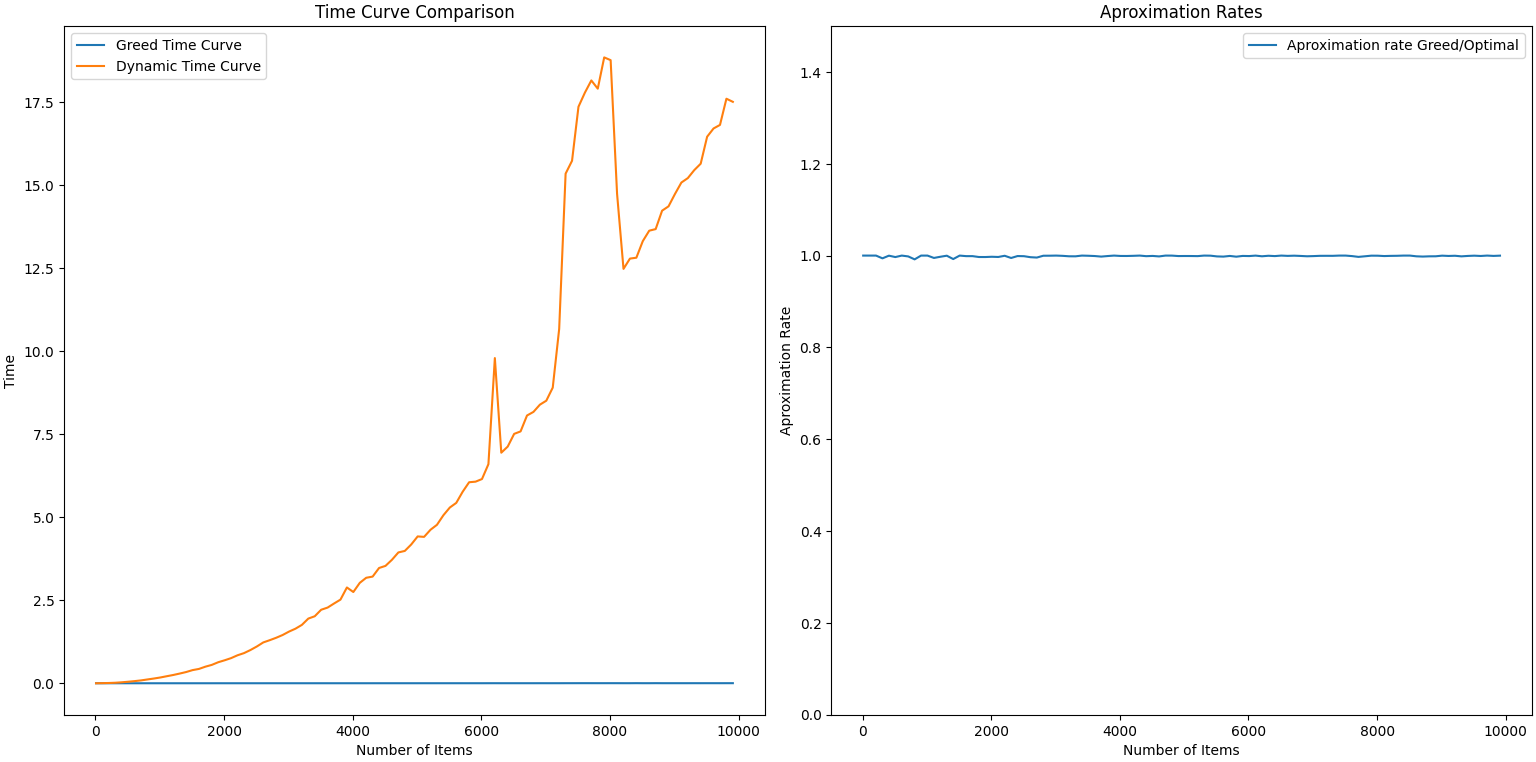
\includegraphics[scale = .3]{images/Figure_1.png}\label{Dell g15 execution}

        Como podemos observar, o algoritmo dinâmico possui um crescimento exponencial para esse caso de teste, muito em razão do crescimento da curva para esse caso de teste um tanto limítrofe, considerando que a matriz de operações a serem realizadas acaba crescendo em $O(n^2)$ em razão da forma como realizamos os testes, sempre n itens e n peso máximo.\\
        A taxa de aproximação permanece aproximadamente constante, confortavelmente próxima de 1.\\
        Uma anomalia nesses dados obtidos pode ser observada em cerca de 6000 itens e 8000 itens, com a execução tomando muito muito mais tempo que o normal. Isso pode talvez ser explicado pelo aquecimento do hardware de testes, mas é incerto o que causou esse súbito aumento no tempo de rodagem. \\
        
    \subsection{SteamDeck}
        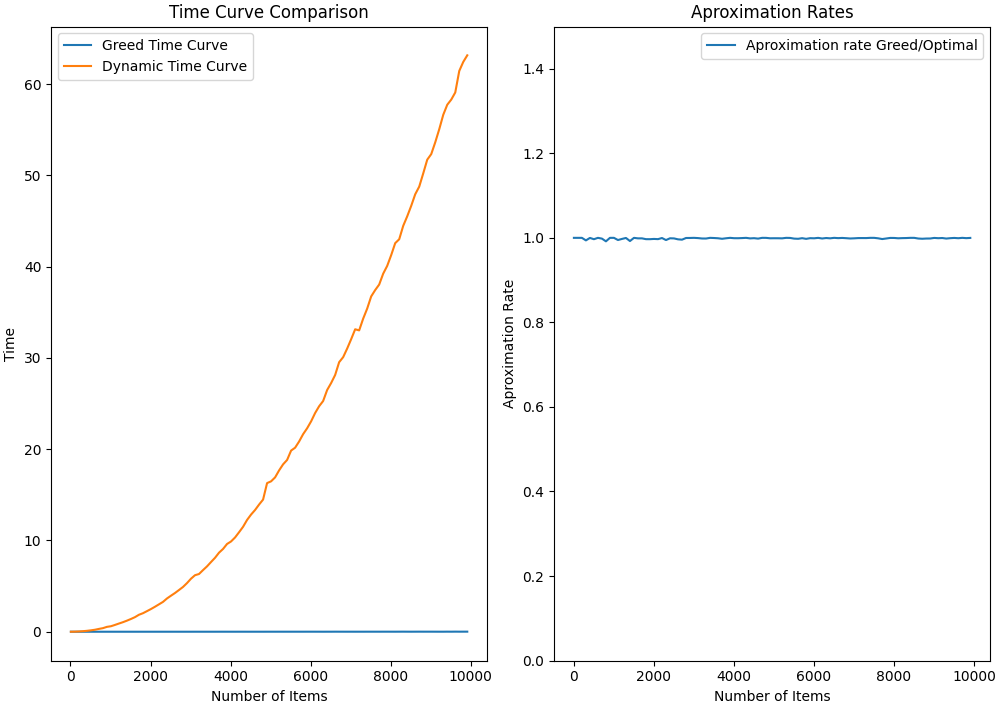
\includegraphics[scale = 0.45]{images/Figure_2.png}\label{SteamDeck execution}
        
        Assim como no teste anterior, o algoritmo dinâmico cresce em $O(n^2)$, e a taxa de aproximação continua aproximadamente constante e próxima de 1.\\
        O tempo do dinâmico, por conta do processamento mais lento do processador em modo single core, acaba ultrapassando marca de um minuto.\\

\section{Conclusão}
    O algoritmo dinâmico, apesar de ótimo, apresentou crescimento do consumo de memória e tempo altamente superiores ao algoritmo de aproximação ganancioso. Isso demonstra certas vantagens e desvantagens sobre as famílias de algoritmo.\\
    Algoritmos dinâmicos são ideais para computação científica e certas aplicações financeiras logísticas, especialmente envolvendo transporte de recursos, mas podem apresentar um tempo de execução elevado e um consumo de memória impraticável para um hardware limitado ou antigo.\\
    Aproximar tais algoritmos pode ser ideal para situações onde uma resposta rápida é necessária ou no mínimo ideal, especialmente para aplicações de tempo real, como já citado, jogos eletrônicos, onde determinados algoritmos têm não mais que o tempo de um frame para retornar uma resposta e protelar a resposta impacta diretamente na usabilidade do software.\\
    Ademais, devido às restrições de data limite para a entrega desse relatório, outros algoritmos poderiam ter sido implementados e a rodagem de tais algoritmos poderia ter se beneficiado de uma gama maior de sistemas operacionais testados em outros hardwares. Caso o leitor busque expandir no curto trabalho aqui feito, esse seria um excelente começo.\\
    Outras formas de expandir o trabalho seria ao implementar outros tipos de aproximação ou otimizações ao algoritmo ótimo, observado que esse relatório é um tanto curto nesse quesito.
    No mais, a dupla agradece a leitura. 
% amongus sussy baka >:3 
% ඞ
% VIOLENCE! - locvst
% JULIETCHARLIEINDIAINDIAHOTELNOVEMBER - also locvst
\end{document}
